\documentclass[a4paper]{article}

\usepackage[english]{babel}
\usepackage[utf8]{inputenc}
\usepackage{amsmath}
\usepackage{graphicx}
\usepackage{hyperref}
\usepackage[colorinlistoftodos]{todonotes}
\graphicspath{ {images/} }
\begin{document}
\begin{titlepage}
    \begin{center}
        {\large Instituto de Matemática e Estatística - Universidade de São Paulo} \\
        {\large IME-USP} \\[4.9cm]
        {\Huge Computação de Alta Performance} \\[9.9cm]
        \vfill
        {\large SÃO PAULO} \\
        {\large 2008}
    \end{center}
\end{titlepage}

\newpage

\begin{titlepage}
    \begin{center}
        {\large Instituto de Matemática e Estatística - Universidade de São Paulo} \\
        {\large IME-USP} \\[4.9cm]
        {\Huge Computação de Alto Desempenho} \\[4.9cm]
        {\large Monografia - Organização de Computadores } \\
        {\large Professor - Siang Wun Song } \\[2.9cm]
        {\large Fellipe Souto \\
                Gervásio Santos \\ 
                Renato Cordeiro} \\[2.9cm]
        \vfill
        {\large SÃO PAULO} \\
        {\large 2008}
    \end{center}
\end{titlepage}

\tableofcontents

\newpage

\section{Introdução}

No ultimo século a computação passou de uma ferramenta de tarefas pontuais, como cálculos balísticos, para uma de muitos propósitos. Tarefas essas que levavam dias, meses ou até anos para serem computadas passaram a apresentar uma resposta computacional em minutos ou segundos. Em face disso a demanda por computação só aumentou ao longo dos anos,  problemas cada vez maiores começaram a ser modelados para serem tratados computacionalmente, temos como grande exemplo desse bem sucedido casamento de conceitos a previsão moderna do tempo.

A computação de alto desempenho sempre esteve na vanguarda da evolução computacional. Ela ditou tendências de hardware e software que perduram até hoje e que refletem o atual estado da arte, como a arquitetura de Von Neumann, o uso de circuitos integrados, múltiplos cores em uma mesma pastilhas, uso de linguagens de baixo nível para tarefas que exigem velocidade, placas aceleradoras dentre outras.

Daremos ao longo deste trabalho um apanhado geral sobre a área de computação de alta performance, discutindo sobre sua história, evolução, tecnologias atuais, dificuldades e desafios encontrados e algumas previsões para o estado futuro da computação.

\section{A história da computação de alta performance}

A história da computação de alta performance está intimamente ligada com a inovação e a com a necessidade de solucionar novos, ou mesmo velhos, problemas. Podemos dividir a história em quatro partes:

\subsection{O começo: os anos 50 e 60}

Acredita-se que o termo Super Computing sido utilizado pela primeira vez no jornal New York World em 1929 para se referir a uma máquina de tabular construída pela IBM para a universidade de Columbia.

A empresa CDC (Control Data Corporation) foi pioneira na criação de supercomputadores. Em 1960 foi criado o CDC-1604, desenhado pelo engenheiro elétrico Seymour Cray, este computador foi considerado o mais rápido do mundo na sua época, sendo utilizado principalmente para fins militares. Nos anos de 1964 foi lançado o CDC-6600 também desenhado por Cray. Este computador teve um acréscimo de velocidade separando a unidade de processando (CPU) das unidades de processamento periférico (PP), permitindo que a CPU lidasse apenas com os cálculos e as PP's com a entrada e saída de de dados. O primeiro modelo lançado do CDC-6600  era utilizado pelo laboratório CERN para analisar milhões de foto tiradas dentro de uma câmara de bolhas.
Em 1972 Cray deixou a CDC para fundar sua própria companhia, começando assim a segunda parte da história da computação de alto desempenho

\subsection{A era Cray: metade dos anos 70 e anos 80}

Em 1976 Cray desenvolveu o Cray-1, que se tornaria o supercomputador mais bem sucedido da história. Ele usava circuitos integrados e tinha processamento vetorial de instruções.

\begin{figure}[h]
\centering
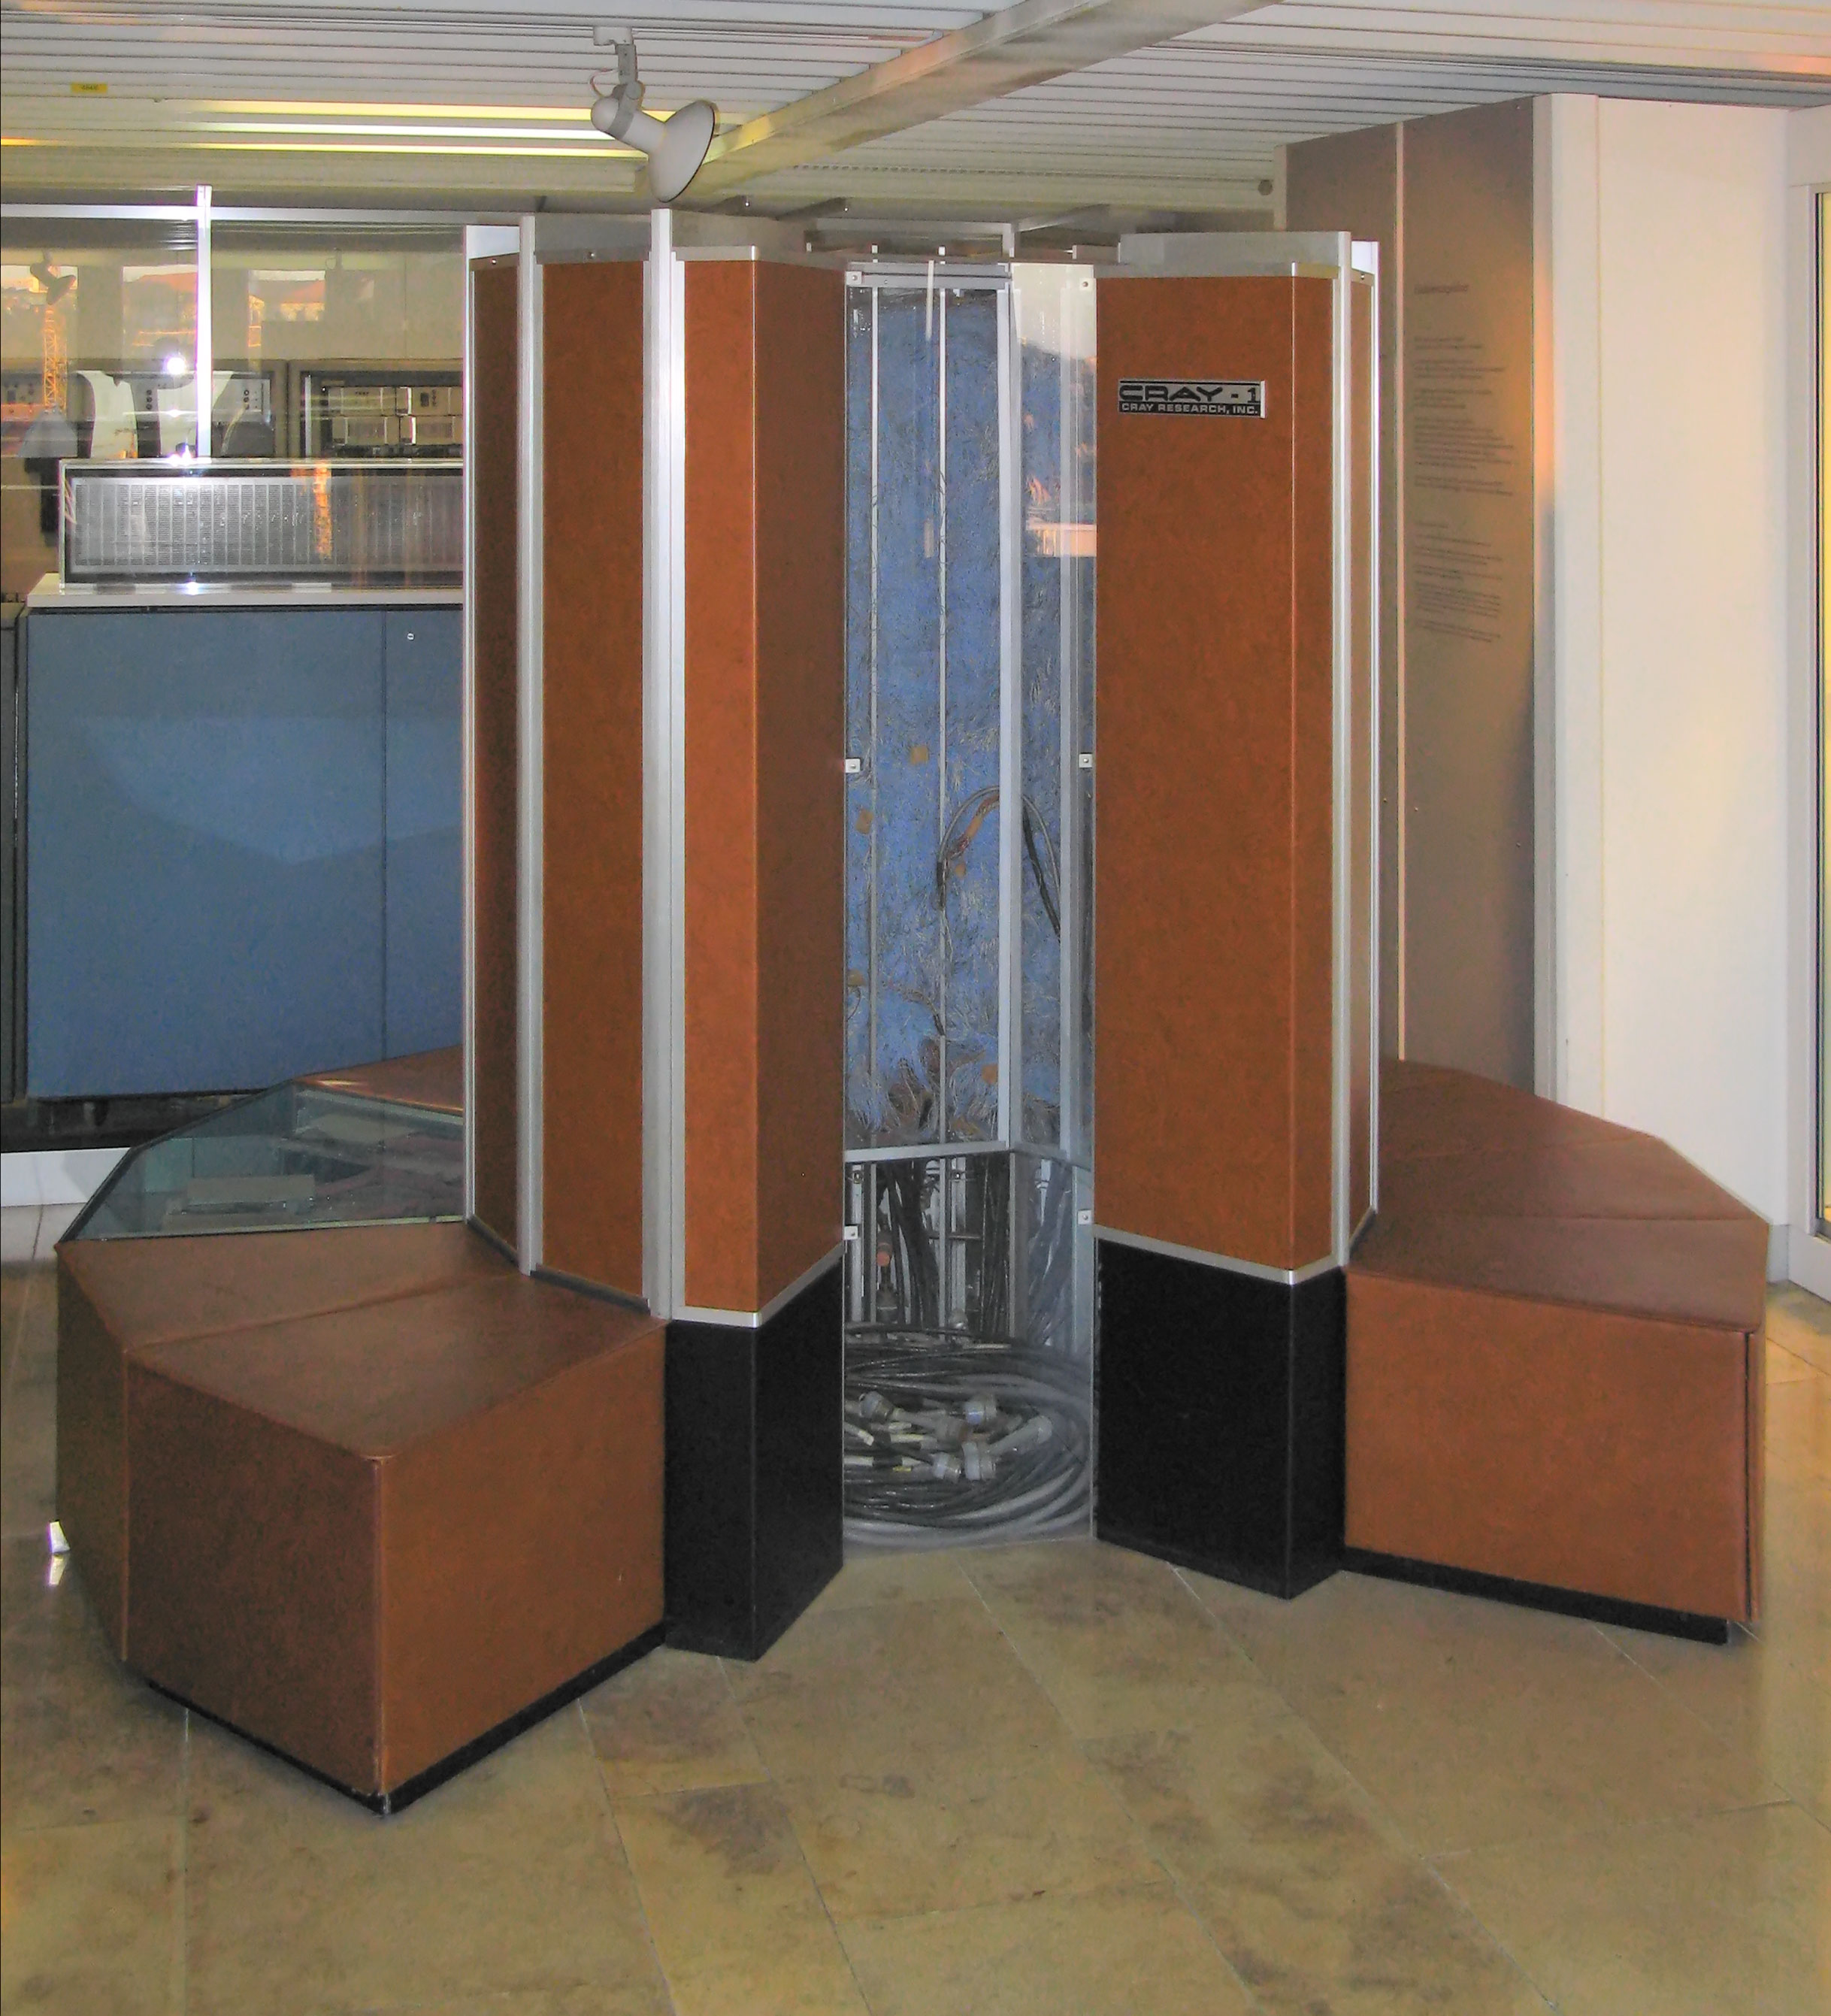
\includegraphics[scale=0.1]{cray1}
\caption{Cray 1 preservado no Deutsches Musem (\textit{fonte: Wikipedia})}
\end{figure}
Em 1985 tivemos o Cray-2, um supercomputador de quatro processadores refrigerados  em um tanque de fluor-inerte, que era constantemente bombeado enquanto ele funcionava.

Cray começou a trabalhar com computação maciçamente paralela nos anos de 1990, mas acabou morrendo em um acidente de carro no ano de 1996, antes de poder colher os frutos  da sua pesquisa. Essa mudança de paradigma marca a terceira parte da história.

\subsection{Processamento massivo: os anos 90}

O Cray-2, que quebrou as fronteiras da supercomputação nos anos 80, possuía apenas quatro processadores. Nos anos 90 um novo paradigma de colocar milhares de processadores em um mesmo computador começou a entrar em cena, em grande parte impulsionada pelo desenvolvimento dos supercomputadores japoneses.

Podemos citar os notáveis supercomputadores japoneses, o primeiro era o Fujitsu Numerical Wind Tunnel com 166 processadores vetoriais e pico de 1.6 gigaflops por processador, ficando em primeiro lugar dos mais rápidos no ano de 94. Em seguida temos o Hitachi SR2201, que obteve o primeiro lugar em 96 com um pico de 600 gigaflops utilizando 2048 processadores.

Utilizando a arquitetura Paragon da Intel, o Intel ASCI Red, fabricado nos Estados Unidos, alcançou o topo do pódio dos supercomputadores no final do século. Ele era composto por mais de 9000 nodos que utilizavam processadores Pentium Pro, comuns em computadores pessoais da época. O ASCI Red foi o primeiro computador a ultrapassar a barreira do teraflop no benchmark LINPACK, atingindo um total de 2 teraflops.

Essa quebra de barreira marca a ultima parte da história e o estado atual em que nos encontramos.
\begin{figure}[h]
\centering
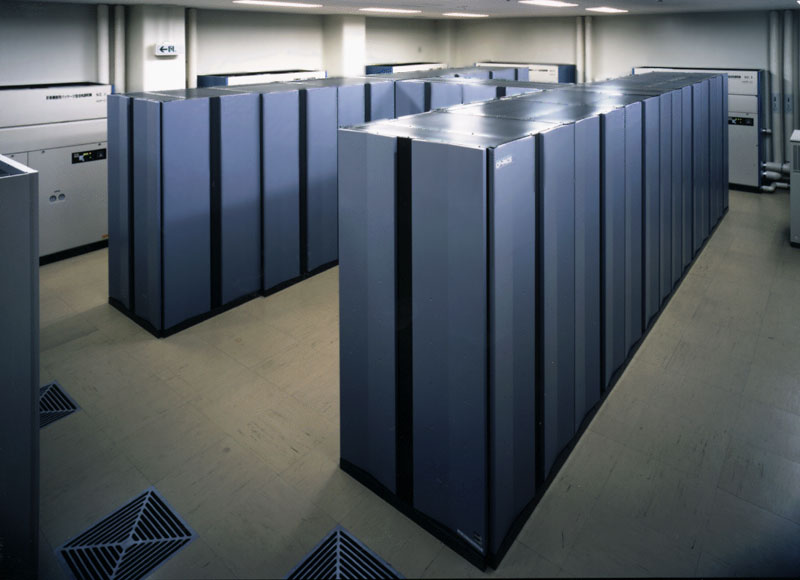
\includegraphics[scale=0.3]{hitachi1}
\caption{Um Hitachi SR2201 (\textit{fonte: ExtremeTech})}
\end{figure}
\subsection{A era Petaflop e o século 21}

A evolução da supercomputação no século 21 deu grandes saltos, mas também teve que amargar velhos problemas. A eficiência computacional cresceu, juntamente com o consumo de energia e o calor gerado no processo.

Ter um supercomputador acabou se tornando uma questão vital para certos países e empresas, seja no âmbito político ou comercial. A China tornou-se um notável exemplo  de desenvolvimento na área, tendo um representante da lista TOP500 em 51$^{\circ}$ em Junho de 2003. Em Novembro de 2003 ela alcançou 14$^{\circ}$ e a 10$^{\circ}$ em Junho de 2004. Em 2010 ela atingiu o primeiro lugar com o Tianhen-1, o maior supercomputador do mundo, com 2.5 petaflops de performance, que permanece até o ano de 2014 na mesma posição.

Utilizando a lista do site TOP500 podemos ter uma noção da rápida evolução que os supercomputadores obtiveram nos últimos 20 anos. É notável perceber que em um diferença máxima de 10 anos o computador mais rápido do mundo tornasse o ultimo colocado da lista.

\section{A arquitetura de um supercomputador}

Analisar a arquitetura de um computador é uma tarefa com diversas abordagens diferentes. Pode-se analisar através da memória, conexão entre os computadores, propósito da arquitetura, performance entre outras. Faremos uma breve análise de todas essas.

\subsection{Instruções e dados}
Para essa abordagem pode-se utilizar a taxonomia de Flynn, que categoriza cada computador de acordo com o número de canais de instruções e canais de dados. Podemos ter as seguintes taxonomias : 

\begin{enumerate}

\item {Single Instruction Single Data(SISD) - Tipo mais básico, com apenas um instrução e uma entrada de dados por vez, acaba não fazendo uso do paralelismo durante a execução. Computadores antigos são um exemplo.

\begin{figure}[h]
\centering
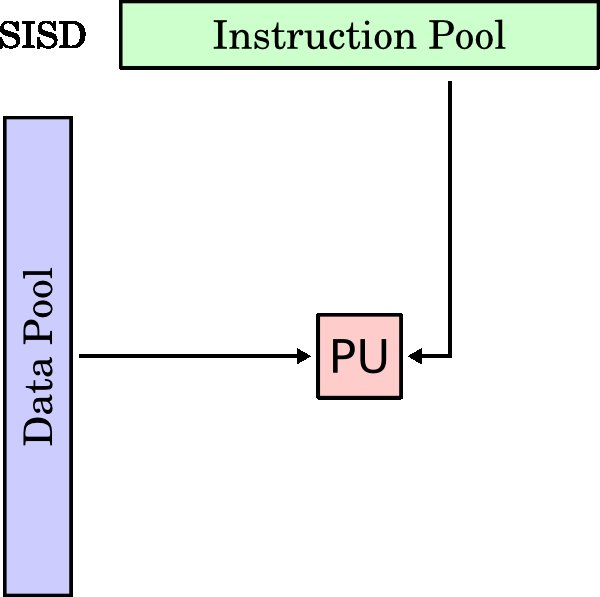
\includegraphics[scale=0.5]{SISD}
\caption{Esquema SISD (\textit{fonte: Wikipedia})}
\end{figure}
}

\item {Single Instruction Multiple Data(SIMD) – Uma instrução é transmitida para diversos processadores, onde cada um possuí seu canal de dados. Placas gráficas são um exemplo.

\begin{figure}[h]
\centering
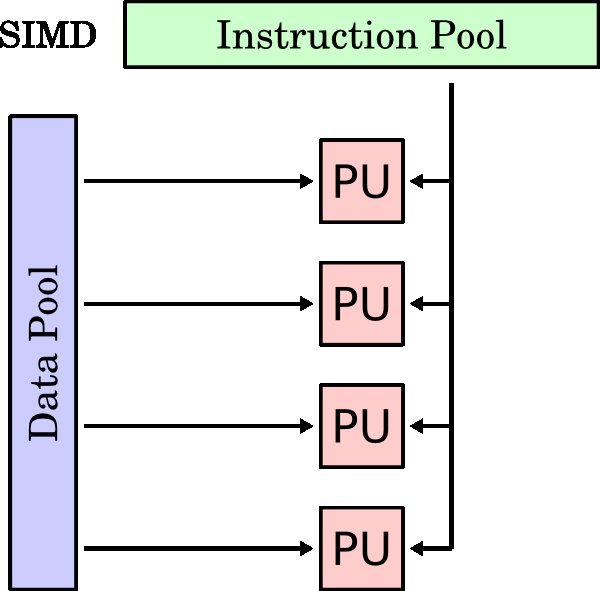
\includegraphics[scale=0.5]{SIMD}
\caption{Esquema SIMD (\textit{fonte: Wikipedia})}
\end{figure}}

\item {Multiple Instruction Single Data(MISD) – Diversas instruções são executadas com apenas um canal de dados. Essa abordagem é utilizada em sistemas heterogêneos para detecção de falha, já que todos os sistemas receberão as mesmas instruções e entradas, tendo assim que gerar as mesmas saídas.
\begin{figure}[h]
\centering
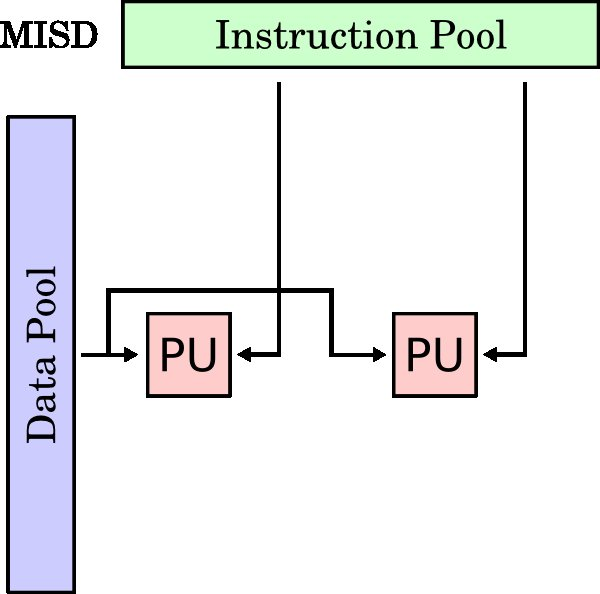
\includegraphics[scale=0.5]{MISD}
\caption{Esquema MISD (\textit{fonte: Wikipedia})}
\end{figure}}

\item {Multiple Instruction Multiple Data(MIMD) – É a principal taxonomia utilizada hoje para atingir paralelismo. Cada processador tem seu canal de dados e seu conjunto de instruções, podendo ainda ter seu próprio segmento de memória ou compartilhar com os outros. Por ser a principal tecnologia de paralelismo será dado maior enfase nela.
\begin{figure}[h]
\centering
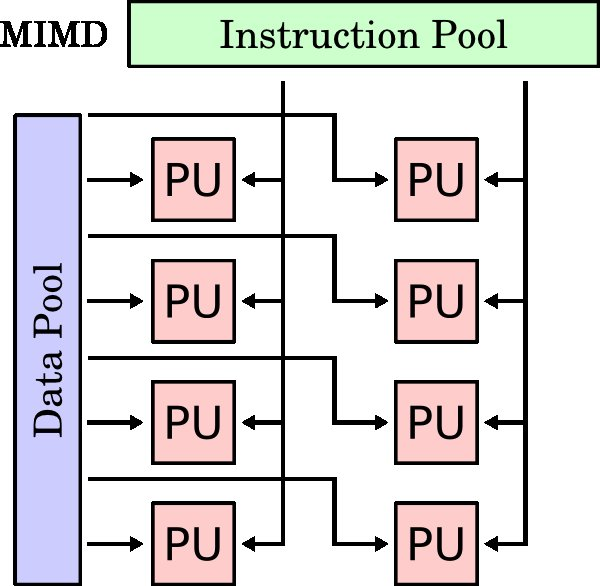
\includegraphics[scale=0.5]{MIMD}
\caption{Esquema MIMD (\textit{fonte: Wikipedia})}
\end{figure}}
\end{enumerate}

\subsection{Memória na arquitetura MIMD}

A Arquitetura MIMD é comumente decomposta em função da sua organização de memória, podendo ser compartilhada ou distribuída.

\subsubsection{Memória compartilhada}

Neste modelo cada processador compartilha um endereço de memória comum com os outros, através da leitura e escrita em variáveis compartilhadas. Esse tipo de memória ainda pode ser dividido em dois grupos , as SMP e as NUMA.

SMP, ou symmetric multiprocessors, é um tipo de memória compartilhada onde todos os processadores conseguem acessar os dados na mesma velocidade. Isso permite que o programador não se preocupe com a distribuição de estruturas de dados ao longo dos processadores. Entretanto esse modelo não escala muito bem, sendo indicado para uma quantidade pequena de processadores.

\begin{figure}[h]
\centering
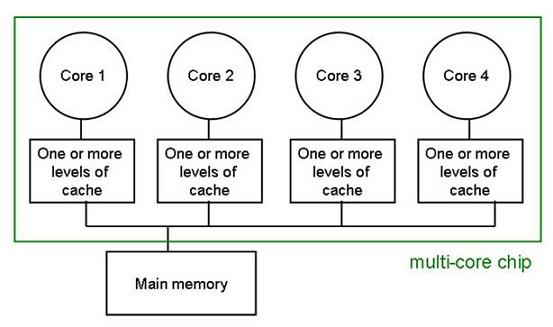
\includegraphics[scale=0.6]{memcomp}
\caption{Esquema de memória compartilhada}
\end{figure}

NUMA, nonuniform memory acess, nesse modelo existem diversos processadores que possuem endereçamento para todos segmentos de memória, porém existe uma diferença de distância entre certos segmentos de memória e um dado processador, o que pode tornar a leitura de algum trecho não uniforme comparado a um outro processador que está tentando ler o mesmo dado. Esse problema de acesso não uniforme pode ser abrandado com o uso de cache nos processadores.


\subsubsection{Memória distribuída}

Neste modelo cada processo tem seu segmento de memória própria e se comunica com os outros processos através do envio de mensagens. A forma como cada interconexão será feita dentro da rede de processos e a tecnologia utilizada são determinante para velocidade na comunicação, podendo ser quase tão rápida quanto a memória compartilhada.
\begin{figure}[h]
\centering
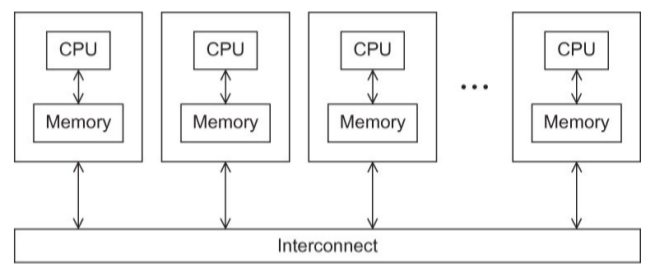
\includegraphics[scale=0.5]{memdist}
\caption{Esquema de memória distribuída}
\end{figure}
Podemos dividir esse tipo de sistema em duas classes, processadores maciçamente paralelizados e clusters. 

Em processadores maciçamente paralelizados, tanto os processadores como a infraestrutura da rede são altamente acoplados e utilizados em uma tarefa bem específica. Esse tipo de sistema tem uma boa escalabilidade e pode comportar milhares de processadores em um único sistema.

Ao passo que os clusters tem uma definição mais abrangente, podendo ser um sistema composto por maquinas e conexões de redes comerciais rodando um dado sistema operacional. Uma maquina mestre distribui tarefa ao longo da rede e colhe depois os dados processados. Um famoso uso da ideia de clusters é o projeto SETI@HOME, que busca evidências de vida extraterrestre analisando sinais de rádio. Os dados são processados por usuários espalhados pelo mundo e enviados de volta para o SETI.

\subsubsection{Sistema híbrido}
São sistemas que tentam explorar o melhor de cada tecnologia para assim atingir o máximo de performance. Um exemplo seria um cluster de nós em arquitetura NUMA onde cada subconjunto é um SMP. Grande parte dos supercomputadores da atualidade são sistemas hídridos.
\newpage

%Parte das referências

\begin{thebibliography}{9}

\bibitem{patterns}
   Timothy G. Mattson, Beverly A. Sanders, Berna L. Massingill 
  \emph{Patterns for Parallel Programming}.
  Addison Wesley,
  1nd edition,
  2013.

\bibitem{highly}
   George S. Almasi, Allan Gottlieb
  \emph{Highly Parallel Computing}.
  Addison Wesley,
  1nd edition,
  1994.

\bibitem{advanced}
    Hesham El-Rewini, Mostafa Abd-El-Barr
  \emph{Advanced Computer Architecture and Parallel Processing}.
  John Wiley \& Sons,
  1nd edition,
  2005.

\bibitem{superwiki}
    Wikipedia contributors,
  \emph{Superercomputer}.
  Wikipedia, The Free Encyclopedia, http://en.wikipedia.org/w/index.php?title=Supercomputer\&oldid=637198749 (accessed November 29, 2014).

\end{thebibliography}

\end{document}